%%%%%%%%%%%%%%%%%%%%%%%%%%%%%%%%%%%%%%%%%%%%%%%%%%%%%%%%%%%%
%%  This Beamer template was created by Cameron Bracken.
%%  Anyone can freely use or modify it for any purpose
%%  without attribution.
%%
%%  Last Modified: January 9, 2009
%%

\documentclass[xcolor=x11names,compress]{beamer}

%% General document %%%%%%%%%%%%%%%%%%%%%%%%%%%%%%%%%%
\usepackage{graphicx}
\usepackage{tikz}
\usepackage[latin1]{inputenc}  
\usetikzlibrary{decorations.fractals}
%%%%%%%%%%%%%%%%%%%%%%%%%%%%%%%%%%%%%%%%%%%%%%%%%%%%%%


%% Beamer Layout %%%%%%%%%%%%%%%%%%%%%%%%%%%%%%%%%%
\useoutertheme[subsection=false,shadow]{miniframes}
\useinnertheme{default}
%\usefonttheme{serif}
\usepackage{helvet}

\setbeamerfont{title like}{shape=\scshape}
\setbeamerfont{frametitle}{shape=\scshape}

\definecolor{playGreen}{RGB}{146,209,61}
\definecolor{textGrey}{RGB}{69,69,69}
\definecolor{backgroundColor}{RGB}{230,230,230}

\setbeamercolor*{lower separation line head}{bg=playGreen} 
\setbeamercolor*{normal text}{fg=textGrey,bg=backgroundColor} 
\setbeamercolor*{alerted text}{fg=red} 
\setbeamercolor*{example text}{fg=black} 
\setbeamercolor*{structure}{fg=black} 
 
\setbeamercolor*{palette tertiary}{fg=black,bg=black!10} 
\setbeamercolor*{palette quaternary}{fg=black,bg=black!10} 


\renewcommand{\(}{\begin{columns}}
\renewcommand{\)}{\end{columns}}
\newcommand{\<}[1]{\begin{column}{#1}}
\renewcommand{\>}{\end{column}}
%%%%%%%%%%%%%%%%%%%%%%%%%%%%%%%%%%%%%%%%%%%%%%%%%%

\setbeamertemplate{section page}
{
  \begin{centering}
    \vskip1em\par
    \begin{beamercolorbox}[sep=4pt,center]{part title}
      \usebeamerfont{section title}\insertsection\par
    \end{beamercolorbox}
  \end{centering}
}

\AtBeginSection{\frame{\sectionpage}}



\begin{document}


%%%%%%%%%%%%%%%%%%%%%%%%%%%%%%%%%%%%%%%%%%%%%%%%%%%%%%
%%%%%%%%%%%%%%%%%%%%%%%%%%%%%%%%%%%%%%%%%%%%%%%%%%%%%%
{
\setbeamercolor{background canvas}{bg=playGreen}
\setbeamercolor{title}{fg=white,bg=playGreen} 
\begin{frame}
\title{\textbf{MVC and MVP patterns with Play! Framework and Backbone.js}}
%\subtitle{SUBTITLE}
\author{
	Alberto Garc�a Garc�a\\
	{\it $<$ agg180@alu.ua.es $>$}\\
}
\date{
	
\includegraphics[height=30px]{play.png} %~ ~ 
\includegraphics[height=20px]{backbone.png}
	\\
	\vspace{1cm}
	\normalsize{\today}
}
\titlepage
\end{frame}
}

%%%%%%%%%%%%%%%%%%%%%%%%%%%%%%%%%%%%%%%%%%%%%%%%%%%%%%
%%%%%%%%%%%%%%%%%%%%%%%%%%%%%%%%%%%%%%%%%%%%%%%%%%%%%%

\begin{frame}{Table of Contents}
\tableofcontents
\end{frame}

%%%%%%%%%%%%%%%%%%%%%%%%%%%%%%%%%%%%%%%%%%%%%%%%%%%%%%
%%%%%%%%%%%%%%%%%%%%%%%%%%%%%%%%%%%%%%%%%%%%%%%%%%%%%%

\section{\scshape Introduction}
\subsection{\scshape Trends}
\begin{frame}
\frametitle{Trends}
	\begin{itemize}
		\item{Enterprises's needs lead the market.}
		\item{Offering services: SOA wins.}
		\item{The web changes the status quo.}
		\item{SOA is not web compliant.}
		\item{Exposing services through the web requires extra effort.}
		\item{The game changes: new possibilities and challenges.}
	\end{itemize}
\end{frame}

%%%%%%%%%%%%%%%%%%%%%%%%%%%%%%%%%%%%%%%%%%%%%%%%%%%%%%
%%%%%%%%%%%%%%%%%%%%%%%%%%%%%%%%%%%%%%%%%%%%%%%%%%%%%%

\subsection{\scshape Challenges}
\begin{frame}
\frametitle{Challenges}
	\begin{itemize}
		\item{Real time data has to be pushed.}
		\item{Huge amounts of data.}
		\item{Need for scalability and integration.}
		\item{Easy integration and accessibility.}
		\item{Interoperability.}
	\end{itemize}
\end{frame}

%%%%%%%%%%%%%%%%%%%%%%%%%%%%%%%%%%%%%%%%%%%%%%%%%%%%%%
%%%%%%%%%%%%%%%%%%%%%%%%%%%%%%%%%%%%%%%%%%%%%%%%%%%%%%

\subsection{\scshape Addressing the challenges}
\begin{frame}
\frametitle{Addressing the challenges}
	\begin{itemize}
		\item{Embrace the internet.}
		\begin{itemize}
			\item{HTTP Protocol}
			\item{HTML5}
			\item{XML/JSON}
			\item{Javascript}
			\item{CSS}
		\end{itemize}
		\item{Paradigm shift: client-side.}
		\item{Simplicity.}
		\item{A framework to rule them all.}
	\end{itemize}
\end{frame}

%%%%%%%%%%%%%%%%%%%%%%%%%%%%%%%%%%%%%%%%%%%%%%%%%%%%%%
%%%%%%%%%%%%%%%%%%%%%%%%%%%%%%%%%%%%%%%%%%%%%%%%%%%%%%

\section{\scshape Play! Framework}
\subsection{What is Play! Framework?}
\begin{frame}{What is Play! Framework?}
	\begin{itemize}
		\item{A web framework focused on:}
		\begin{itemize}
			\item{Simplicity.}
			\item{Productivity.}
			\item{Scalability.}
			\item{Designed for the modern web.}
			\begin{itemize}
				\item{Concentrate on server-side.}
				\item{Delegate AMAP to the client.}
			\end{itemize}
			\item{Embrace internet standards.}
			\item{Java and Scala.}
			\item{RESTful architecture web applications.}
			\item{Model-View-Controller.}
		\end{itemize}
	\end{itemize}
\end{frame}

%%%%%%%%%%%%%%%%%%%%%%%%%%%%%%%%%%%%%%%%%%%%%%%%%%%%%%
%%%%%%%%%%%%%%%%%%%%%%%%%%%%%%%%%%%%%%%%%%%%%%%%%%%%%%

\subsection{RESTful Architecture}
\begin{frame}{RESTful architecture}
	\begin{itemize}
		\item{Implemented using HTTP and REST principles.}
		\item{Representational state transfer (REST) principles:}
		\begin{itemize}
			\item{Uniform interface.}
			\item{Stateless.}
			\item{Caching.}
			\item{Layers.}
			\item{Code on demand.}
		\end{itemize}
		\item{Goals:}
		\begin{itemize}
			\item{Performance.}
			\item{Scalability.}
			\item{Portability.}
			\item{Reliability.}
			\item{SIMPLICITY.}
		\end{itemize}
	\end{itemize}
\end{frame}

%%%%%%%%%%%%%%%%%%%%%%%%%%%%%%%%%%%%%%%%%%%%%%%%%%%%%%
%%%%%%%%%%%%%%%%%%%%%%%%%%%%%%%%%%%%%%%%%%%%%%%%%%%%%%

\subsection{The MVC application model}
\begin{frame}{The MVC application model}
	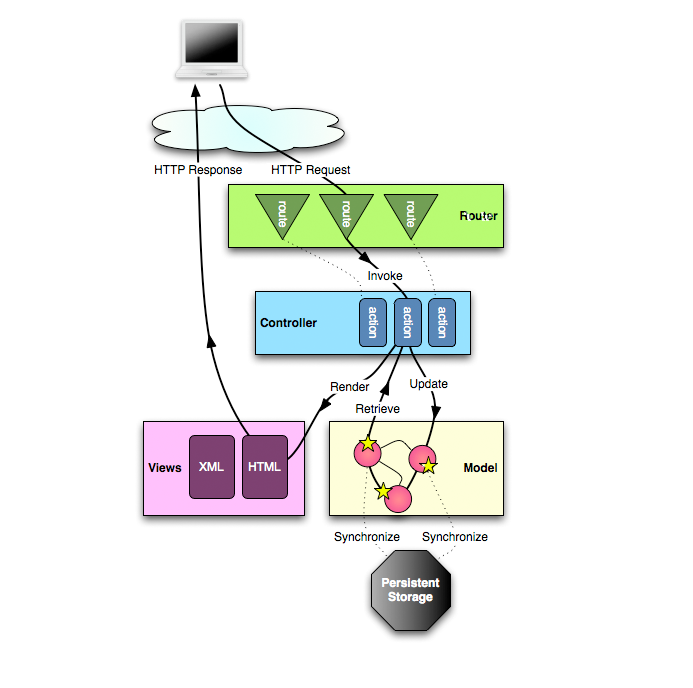
\includegraphics[height=200px]{diagrams_path.png}
\end{frame}

%%%%%%%%%%%%%%%%%%%%%%%%%%%%%%%%%%%%%%%%%%%%%%%%%%%%%%
%%%%%%%%%%%%%%%%%%%%%%%%%%%%%%%%%%%%%%%%%%%%%%%%%%%%%%

\section{\scshape Backbone.js}
\subsection{What is Backbone.js?}
\begin{frame}{What is Backbone.js?}

\end{frame}

%%%%%%%%%%%%%%%%%%%%%%%%%%%%%%%%%%%%%%%%%%%%%%%%%%%%%%
%%%%%%%%%%%%%%%%%%%%%%%%%%%%%%%%%%%%%%%%%%%%%%%%%%%%%%

\section*{\scshape References}
\begin{frame}[allowframebreaks]
	\normalsize
	\nocite{PlayForJava}
	\nocite{PlayForScala}
	\nocite{PlayFrameworkCookbook}
	\frametitle{References}
	\bibliographystyle{amsalpha}
	\bibliography{biblio.bib}
\end{frame}

\end{document}